\batchmode
\documentclass[twoside]{book}

% Packages required by doxygen
\usepackage{fixltx2e}
\usepackage{calc}
\usepackage{doxygen}
\usepackage[export]{adjustbox} % also loads graphicx
\usepackage{graphicx}
\usepackage[utf8]{inputenc}
\usepackage{makeidx}
\usepackage{multicol}
\usepackage{multirow}
\PassOptionsToPackage{warn}{textcomp}
\usepackage{textcomp}
\usepackage[nointegrals]{wasysym}
\usepackage[table]{xcolor}

% Font selection
\usepackage[T1]{fontenc}
\usepackage[scaled=.90]{helvet}
\usepackage{courier}
\usepackage{amssymb}
\usepackage{sectsty}
\renewcommand{\familydefault}{\sfdefault}
\allsectionsfont{%
  \fontseries{bc}\selectfont%
  \color{darkgray}%
}
\renewcommand{\DoxyLabelFont}{%
  \fontseries{bc}\selectfont%
  \color{darkgray}%
}
\newcommand{\+}{\discretionary{\mbox{\scriptsize$\hookleftarrow$}}{}{}}

% Page & text layout
\usepackage{geometry}
\geometry{%
  a4paper,%
  top=2.5cm,%
  bottom=2.5cm,%
  left=2.5cm,%
  right=2.5cm%
}
\tolerance=750
\hfuzz=15pt
\hbadness=750
\setlength{\emergencystretch}{15pt}
\setlength{\parindent}{0cm}
\setlength{\parskip}{3ex plus 2ex minus 2ex}
\makeatletter
\renewcommand{\paragraph}{%
  \@startsection{paragraph}{4}{0ex}{-1.0ex}{1.0ex}{%
    \normalfont\normalsize\bfseries\SS@parafont%
  }%
}
\renewcommand{\subparagraph}{%
  \@startsection{subparagraph}{5}{0ex}{-1.0ex}{1.0ex}{%
    \normalfont\normalsize\bfseries\SS@subparafont%
  }%
}
\makeatother

% Headers & footers
\usepackage{fancyhdr}
\pagestyle{fancyplain}
\fancyhead[LE]{\fancyplain{}{\bfseries\thepage}}
\fancyhead[CE]{\fancyplain{}{}}
\fancyhead[RE]{\fancyplain{}{\bfseries\leftmark}}
\fancyhead[LO]{\fancyplain{}{\bfseries\rightmark}}
\fancyhead[CO]{\fancyplain{}{}}
\fancyhead[RO]{\fancyplain{}{\bfseries\thepage}}
\fancyfoot[LE]{\fancyplain{}{}}
\fancyfoot[CE]{\fancyplain{}{}}
\fancyfoot[RE]{\fancyplain{}{\bfseries\scriptsize Generated by Doxygen }}
\fancyfoot[LO]{\fancyplain{}{\bfseries\scriptsize Generated by Doxygen }}
\fancyfoot[CO]{\fancyplain{}{}}
\fancyfoot[RO]{\fancyplain{}{}}
\renewcommand{\footrulewidth}{0.4pt}
\renewcommand{\chaptermark}[1]{%
  \markboth{#1}{}%
}
\renewcommand{\sectionmark}[1]{%
  \markright{\thesection\ #1}%
}

% Indices & bibliography
\usepackage{natbib}
\usepackage[titles]{tocloft}
\setcounter{tocdepth}{3}
\setcounter{secnumdepth}{5}
\makeindex

% Hyperlinks (required, but should be loaded last)
\usepackage{ifpdf}
\ifpdf
  \usepackage[pdftex,pagebackref=true]{hyperref}
\else
  \usepackage[ps2pdf,pagebackref=true]{hyperref}
\fi
\hypersetup{%
  colorlinks=true,%
  linkcolor=blue,%
  citecolor=blue,%
  unicode%
}

% Custom commands
\newcommand{\clearemptydoublepage}{%
  \newpage{\pagestyle{empty}\cleardoublepage}%
}

\usepackage{caption}
\captionsetup{labelsep=space,justification=centering,font={bf},singlelinecheck=off,skip=4pt,position=top}

%===== C O N T E N T S =====

\begin{document}

% Titlepage & ToC
\hypersetup{pageanchor=false,
             bookmarksnumbered=true,
             pdfencoding=unicode
            }
\pagenumbering{alph}
\pagenumbering{arabic}
\hypersetup{pageanchor=true}

%--- Begin generated contents ---
\chapter{Demo problem\+: Flow in a 2D channel with an oscillating leaflet}
\label{index}\hypertarget{index}{}\hypertarget{index_q}{}\section{A few quick questions...}\label{index_q}
Since {\ttfamily oomph-\/lib} is developed as open-\/source software, any evidence that the code is being downloaded and used is very helpful for us as it helps to justify our continued work on this project.

We would therefore be extremely grateful if you could provide the information requested in the form below. Pressing the \char`\"{}submit\char`\"{} button will get you to the actual download page.

{\bfseries Note\+:} 
\begin{DoxyItemize}
\item All information will be treated as confidential. 
\item If you provide your email address and check the appropriate box we will add you to our mailing list to inform you of upgrades and bug fixes to the code. Rest assured that the mailing list is {\bfseries very low volume} -- we have better things to do than to bombard you with email. 
\item If you still feel reluctant to provide any of the information requested, feel free to enter some dummy input. The form will check that {\bfseries some} information has been entered but entering your name as \char`\"{}\+Joe Cool\char`\"{} is perfectly acceptable -- this is to discourage people from not providing the information simply because they are too lazy to type... 
\end{DoxyItemize}



 







 

 \hypertarget{index_pdf}{}\section{P\+D\+F file}\label{index_pdf}
A \href{../latex/refman.pdf}{\tt pdf version} of this document is available. \end{document}

\chapter{Namespace Index}
\section{Namespace List}
Here is a list of all namespaces with brief descriptions\+:\begin{DoxyCompactList}
\item\contentsline{section}{\hyperlink{namespaceGlobal__Physical__Variables}{Global\+\_\+\+Physical\+\_\+\+Variables} \\*Global variables that represent physical properties }{\pageref{namespaceGlobal__Physical__Variables}}{}
\item\contentsline{section}{\hyperlink{namespaceoomph}{oomph} }{\pageref{namespaceoomph}}{}
\item\contentsline{section}{\hyperlink{namespacePhysical__Variables}{Physical\+\_\+\+Variables} \\*Namespace for the solution of 2D linear shell equation }{\pageref{namespacePhysical__Variables}}{}
\end{DoxyCompactList}

\chapter{Hierarchical Index}
\section{Class Hierarchy}
This inheritance list is sorted roughly, but not completely, alphabetically\+:\begin{DoxyCompactList}
\item Problem\begin{DoxyCompactList}
\item \contentsline{section}{Unstructured\+Solid\+Problem$<$ E\+L\+E\+M\+E\+NT $>$}{\pageref{classUnstructuredSolidProblem}}{}
\end{DoxyCompactList}
\end{DoxyCompactList}

\chapter{Class Index}
\section{Class List}
Here are the classes, structs, unions and interfaces with brief descriptions\+:\begin{DoxyCompactList}
\item\contentsline{section}{\hyperlink{classPMLProblem}{P\+M\+L\+Problem$<$ E\+L\+E\+M\+E\+N\+T $>$} }{\pageref{classPMLProblem}}{}
\item\contentsline{section}{\hyperlink{classGlobalParameters_1_1TestPMLMapping}{Global\+Parameters\+::\+Test\+P\+M\+L\+Mapping} }{\pageref{classGlobalParameters_1_1TestPMLMapping}}{}
\end{DoxyCompactList}

\chapter{File Index}
\section{File List}
Here is a list of all files with brief descriptions\+:\begin{DoxyCompactList}
\item\contentsline{section}{\hyperlink{jeffery__orbit_8cc}{jeffery\+\_\+orbit.\+cc} }{\pageref{jeffery__orbit_8cc}}{}
\item\contentsline{section}{\hyperlink{jeffery__orbit_8txt__doxygenified_8h}{jeffery\+\_\+orbit.\+txt\+\_\+doxygenified.\+h} }{\pageref{jeffery__orbit_8txt__doxygenified_8h}}{}
\item\contentsline{section}{\hyperlink{my__taylor__hood__elements_8h}{my\+\_\+taylor\+\_\+hood\+\_\+elements.\+h} }{\pageref{my__taylor__hood__elements_8h}}{}
\end{DoxyCompactList}

\chapter{Namespace Documentation}
\hypertarget{namespaceGlobal__Physical__Variables}{}\section{Global\+\_\+\+Physical\+\_\+\+Variables Namespace Reference}
\label{namespaceGlobal__Physical__Variables}\index{Global\+\_\+\+Physical\+\_\+\+Variables@{Global\+\_\+\+Physical\+\_\+\+Variables}}


Namespace for physical parameters.  


\subsection*{Functions}
\begin{DoxyCompactItemize}
\item 
Vector$<$ double $>$ \hyperlink{namespaceGlobal__Physical__Variables_afae321364975eb56688ad13abc8ed6b7}{Gravity} (2)
\begin{DoxyCompactList}\small\item\em Gravity vector. \end{DoxyCompactList}\item 
void \hyperlink{namespaceGlobal__Physical__Variables_a87da705b8a46bed337cf5dbdd788b87b}{body\+\_\+force} (const double \&time, const Vector$<$ double $>$ \&x, Vector$<$ double $>$ \&result)
\begin{DoxyCompactList}\small\item\em Functional body force. \end{DoxyCompactList}\item 
void \hyperlink{namespaceGlobal__Physical__Variables_a9780d615ae07c4e00a436ab2973b54e6}{zero\+\_\+body\+\_\+force} (const double \&time, const Vector$<$ double $>$ \&x, Vector$<$ double $>$ \&result)
\begin{DoxyCompactList}\small\item\em Zero functional body force. \end{DoxyCompactList}\end{DoxyCompactItemize}
\subsection*{Variables}
\begin{DoxyCompactItemize}
\item 
double \hyperlink{namespaceGlobal__Physical__Variables_ab814e627d2eb5bc50318879d19ab16b9}{Re} =100
\begin{DoxyCompactList}\small\item\em Reynolds number. \end{DoxyCompactList}\item 
double \hyperlink{namespaceGlobal__Physical__Variables_ab1a845a672b4d74b304639a976dc65c6}{Re\+\_\+inv\+Fr} =100
\begin{DoxyCompactList}\small\item\em Reynolds/\+Froude number. \end{DoxyCompactList}\end{DoxyCompactItemize}


\subsection{Detailed Description}
Namespace for physical parameters. 

\subsection{Function Documentation}
\mbox{\Hypertarget{namespaceGlobal__Physical__Variables_a87da705b8a46bed337cf5dbdd788b87b}\label{namespaceGlobal__Physical__Variables_a87da705b8a46bed337cf5dbdd788b87b}} 
\index{Global\+\_\+\+Physical\+\_\+\+Variables@{Global\+\_\+\+Physical\+\_\+\+Variables}!body\+\_\+force@{body\+\_\+force}}
\index{body\+\_\+force@{body\+\_\+force}!Global\+\_\+\+Physical\+\_\+\+Variables@{Global\+\_\+\+Physical\+\_\+\+Variables}}
\subsubsection{\texorpdfstring{body\+\_\+force()}{body\_force()}}
{\footnotesize\ttfamily void Global\+\_\+\+Physical\+\_\+\+Variables\+::body\+\_\+force (\begin{DoxyParamCaption}\item[{const double \&}]{time,  }\item[{const Vector$<$ double $>$ \&}]{x,  }\item[{Vector$<$ double $>$ \&}]{result }\end{DoxyParamCaption})}



Functional body force. 



Definition at line 62 of file circular\+\_\+driven\+\_\+cavity.\+cc.



References Re\+\_\+inv\+Fr.



Referenced by main().

\mbox{\Hypertarget{namespaceGlobal__Physical__Variables_afae321364975eb56688ad13abc8ed6b7}\label{namespaceGlobal__Physical__Variables_afae321364975eb56688ad13abc8ed6b7}} 
\index{Global\+\_\+\+Physical\+\_\+\+Variables@{Global\+\_\+\+Physical\+\_\+\+Variables}!Gravity@{Gravity}}
\index{Gravity@{Gravity}!Global\+\_\+\+Physical\+\_\+\+Variables@{Global\+\_\+\+Physical\+\_\+\+Variables}}
\subsubsection{\texorpdfstring{Gravity()}{Gravity()}}
{\footnotesize\ttfamily Vector$<$double$>$ Global\+\_\+\+Physical\+\_\+\+Variables\+::\+Gravity (\begin{DoxyParamCaption}\item[{2}]{ }\end{DoxyParamCaption})}



Gravity vector. 



Referenced by main(), and Quarter\+Circle\+Driven\+Cavity\+Problem$<$ E\+L\+E\+M\+E\+N\+T $>$\+::\+Quarter\+Circle\+Driven\+Cavity\+Problem().

\mbox{\Hypertarget{namespaceGlobal__Physical__Variables_a9780d615ae07c4e00a436ab2973b54e6}\label{namespaceGlobal__Physical__Variables_a9780d615ae07c4e00a436ab2973b54e6}} 
\index{Global\+\_\+\+Physical\+\_\+\+Variables@{Global\+\_\+\+Physical\+\_\+\+Variables}!zero\+\_\+body\+\_\+force@{zero\+\_\+body\+\_\+force}}
\index{zero\+\_\+body\+\_\+force@{zero\+\_\+body\+\_\+force}!Global\+\_\+\+Physical\+\_\+\+Variables@{Global\+\_\+\+Physical\+\_\+\+Variables}}
\subsubsection{\texorpdfstring{zero\+\_\+body\+\_\+force()}{zero\_body\_force()}}
{\footnotesize\ttfamily void Global\+\_\+\+Physical\+\_\+\+Variables\+::zero\+\_\+body\+\_\+force (\begin{DoxyParamCaption}\item[{const double \&}]{time,  }\item[{const Vector$<$ double $>$ \&}]{x,  }\item[{Vector$<$ double $>$ \&}]{result }\end{DoxyParamCaption})}



Zero functional body force. 



Definition at line 70 of file circular\+\_\+driven\+\_\+cavity.\+cc.



Referenced by main().



\subsection{Variable Documentation}
\mbox{\Hypertarget{namespaceGlobal__Physical__Variables_ab814e627d2eb5bc50318879d19ab16b9}\label{namespaceGlobal__Physical__Variables_ab814e627d2eb5bc50318879d19ab16b9}} 
\index{Global\+\_\+\+Physical\+\_\+\+Variables@{Global\+\_\+\+Physical\+\_\+\+Variables}!Re@{Re}}
\index{Re@{Re}!Global\+\_\+\+Physical\+\_\+\+Variables@{Global\+\_\+\+Physical\+\_\+\+Variables}}
\subsubsection{\texorpdfstring{Re}{Re}}
{\footnotesize\ttfamily double Global\+\_\+\+Physical\+\_\+\+Variables\+::\+Re =100}



Reynolds number. 



Definition at line 53 of file circular\+\_\+driven\+\_\+cavity.\+cc.



Referenced by Quarter\+Circle\+Driven\+Cavity\+Problem$<$ E\+L\+E\+M\+E\+N\+T $>$\+::\+Quarter\+Circle\+Driven\+Cavity\+Problem().

\mbox{\Hypertarget{namespaceGlobal__Physical__Variables_ab1a845a672b4d74b304639a976dc65c6}\label{namespaceGlobal__Physical__Variables_ab1a845a672b4d74b304639a976dc65c6}} 
\index{Global\+\_\+\+Physical\+\_\+\+Variables@{Global\+\_\+\+Physical\+\_\+\+Variables}!Re\+\_\+inv\+Fr@{Re\+\_\+inv\+Fr}}
\index{Re\+\_\+inv\+Fr@{Re\+\_\+inv\+Fr}!Global\+\_\+\+Physical\+\_\+\+Variables@{Global\+\_\+\+Physical\+\_\+\+Variables}}
\subsubsection{\texorpdfstring{Re\+\_\+inv\+Fr}{Re\_invFr}}
{\footnotesize\ttfamily double Global\+\_\+\+Physical\+\_\+\+Variables\+::\+Re\+\_\+inv\+Fr =100}



Reynolds/\+Froude number. 



Definition at line 56 of file circular\+\_\+driven\+\_\+cavity.\+cc.



Referenced by body\+\_\+force(), and Quarter\+Circle\+Driven\+Cavity\+Problem$<$ E\+L\+E\+M\+E\+N\+T $>$\+::\+Quarter\+Circle\+Driven\+Cavity\+Problem().


\chapter{Class Documentation}
\hypertarget{classChannelWithLeafletProblem}{}\section{Channel\+With\+Leaflet\+Problem$<$ E\+L\+E\+M\+E\+NT $>$ Class Template Reference}
\label{classChannelWithLeafletProblem}\index{Channel\+With\+Leaflet\+Problem$<$ E\+L\+E\+M\+E\+N\+T $>$@{Channel\+With\+Leaflet\+Problem$<$ E\+L\+E\+M\+E\+N\+T $>$}}


Problem class.  


Inheritance diagram for Channel\+With\+Leaflet\+Problem$<$ E\+L\+E\+M\+E\+NT $>$\+:\begin{figure}[H]
\begin{center}
\leavevmode
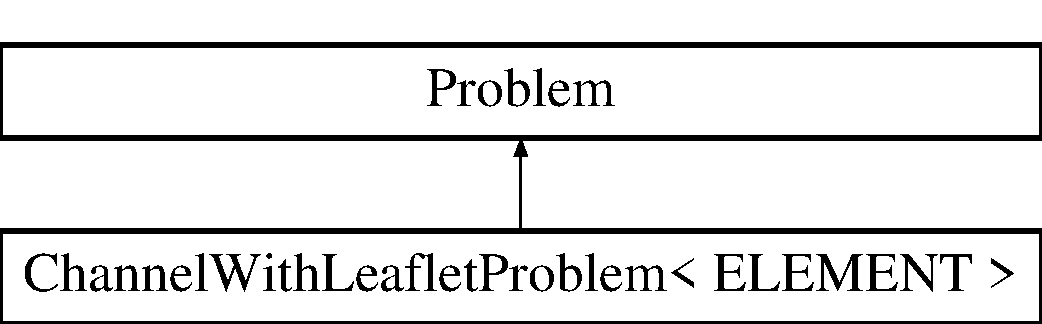
\includegraphics[height=2.000000cm]{classChannelWithLeafletProblem}
\end{center}
\end{figure}
\subsection*{Public Member Functions}
\begin{DoxyCompactItemize}
\item 
\hyperlink{classChannelWithLeafletProblem_a3c5a4c97ec66fe53bc130005c74a47b5}{Channel\+With\+Leaflet\+Problem} (const double \&l\+\_\+left, const double \&l\+\_\+right, const double \&h\+\_\+leaflet, const double \&h\+\_\+tot, const unsigned \&nleft, const unsigned \&nright, const unsigned \&ny1, const unsigned \&ny2, const double \&d\+\_\+x, const double \&d\+\_\+y, const double \&x\+\_\+0, const double \&period)
\begin{DoxyCompactList}\small\item\em Constructor. \end{DoxyCompactList}\item 
\hyperlink{classChannelWithLeafletProblem_a5dec8333d345e4bcaac7fcd5b463eafc}{$\sim$\+Channel\+With\+Leaflet\+Problem} ()
\begin{DoxyCompactList}\small\item\em Destructor (empty) \end{DoxyCompactList}\item 
Refineable\+Algebraic\+Channel\+With\+Leaflet\+Mesh$<$ E\+L\+E\+M\+E\+NT $>$ $\ast$ \hyperlink{classChannelWithLeafletProblem_a023dc7718a98f820e4bc4541150a0c08}{mesh\+\_\+pt} ()
\begin{DoxyCompactList}\small\item\em Overloaded access function to specific mesh. \end{DoxyCompactList}\item 
void \hyperlink{classChannelWithLeafletProblem_a2fcba9dc98f40bbca1919a715fa087d7}{actions\+\_\+after\+\_\+newton\+\_\+solve} ()
\begin{DoxyCompactList}\small\item\em Update after solve (empty) \end{DoxyCompactList}\item 
void \hyperlink{classChannelWithLeafletProblem_a5721dfad66d13a1ae60adce7801dcb12}{actions\+\_\+before\+\_\+newton\+\_\+solve} ()
\begin{DoxyCompactList}\small\item\em Update before solve (empty) \end{DoxyCompactList}\item 
void \hyperlink{classChannelWithLeafletProblem_a7978755f073d950e5012951ced9e455e}{actions\+\_\+after\+\_\+adapt} ()
\begin{DoxyCompactList}\small\item\em Actions after adaptation\+: Pin redundant pressure dofs. \end{DoxyCompactList}\item 
void \hyperlink{classChannelWithLeafletProblem_acef6ec771775162f77295a8f92d695ac}{actions\+\_\+before\+\_\+implicit\+\_\+timestep} ()
\begin{DoxyCompactList}\small\item\em Update the velocity boundary condition on the moving leaflet. \end{DoxyCompactList}\item 
void \hyperlink{classChannelWithLeafletProblem_adb8e1420844f7b40d71beae81111c4d0}{doc\+\_\+solution} (Doc\+Info \&doc\+\_\+info)
\begin{DoxyCompactList}\small\item\em Doc the solution. \end{DoxyCompactList}\end{DoxyCompactItemize}
\subsection*{Private Attributes}
\begin{DoxyCompactItemize}
\item 
Geom\+Object $\ast$ \hyperlink{classChannelWithLeafletProblem_ac32f0451749ec4e85d39246f5823a5f2}{Leaflet\+\_\+pt}
\begin{DoxyCompactList}\small\item\em Pointer to the Geom\+Object. \end{DoxyCompactList}\end{DoxyCompactItemize}


\subsection{Detailed Description}
\subsubsection*{template$<$class E\+L\+E\+M\+E\+NT$>$\newline
class Channel\+With\+Leaflet\+Problem$<$ E\+L\+E\+M\+E\+N\+T $>$}

Problem class. 

Definition at line 151 of file channel\+\_\+with\+\_\+leaflet.\+cc.



\subsection{Constructor \& Destructor Documentation}
\mbox{\Hypertarget{classChannelWithLeafletProblem_a3c5a4c97ec66fe53bc130005c74a47b5}\label{classChannelWithLeafletProblem_a3c5a4c97ec66fe53bc130005c74a47b5}} 
\index{Channel\+With\+Leaflet\+Problem@{Channel\+With\+Leaflet\+Problem}!Channel\+With\+Leaflet\+Problem@{Channel\+With\+Leaflet\+Problem}}
\index{Channel\+With\+Leaflet\+Problem@{Channel\+With\+Leaflet\+Problem}!Channel\+With\+Leaflet\+Problem@{Channel\+With\+Leaflet\+Problem}}
\subsubsection{\texorpdfstring{Channel\+With\+Leaflet\+Problem()}{ChannelWithLeafletProblem()}}
{\footnotesize\ttfamily template$<$class E\+L\+E\+M\+E\+NT $>$ \\
\hyperlink{classChannelWithLeafletProblem}{Channel\+With\+Leaflet\+Problem}$<$ E\+L\+E\+M\+E\+NT $>$\+::\hyperlink{classChannelWithLeafletProblem}{Channel\+With\+Leaflet\+Problem} (\begin{DoxyParamCaption}\item[{const double \&}]{l\+\_\+left,  }\item[{const double \&}]{l\+\_\+right,  }\item[{const double \&}]{h\+\_\+leaflet,  }\item[{const double \&}]{h\+\_\+tot,  }\item[{const unsigned \&}]{nleft,  }\item[{const unsigned \&}]{nright,  }\item[{const unsigned \&}]{ny1,  }\item[{const unsigned \&}]{ny2,  }\item[{const double \&}]{d\+\_\+x,  }\item[{const double \&}]{d\+\_\+y,  }\item[{const double \&}]{x\+\_\+0,  }\item[{const double \&}]{period }\end{DoxyParamCaption})}



Constructor. 

Constructor\+: Pass the length of the domain at the left of the leaflet lleft,the length of the domain at the right of the leaflet lright,the height of the leaflet hleaflet, the total height of the domain htot, the number of macro-\/elements at the left of the leaflet nleft, the number of macro-\/elements at the right of the leaflet nright, the number of macro-\/elements under hleaflet ny1, the number of macro-\/elements above hleaflet ny2,the x-\/displacement of the leaflet d\+\_\+x,the y-\/displacement of the leaflet d\+\_\+y,the abscissa of the origin of the leaflet x\+\_\+0, the period of the moving leaflet. 

Definition at line 214 of file channel\+\_\+with\+\_\+leaflet.\+cc.



References Global\+\_\+\+Physical\+\_\+\+Variables\+::\+Re.

\mbox{\Hypertarget{classChannelWithLeafletProblem_a5dec8333d345e4bcaac7fcd5b463eafc}\label{classChannelWithLeafletProblem_a5dec8333d345e4bcaac7fcd5b463eafc}} 
\index{Channel\+With\+Leaflet\+Problem@{Channel\+With\+Leaflet\+Problem}!````~Channel\+With\+Leaflet\+Problem@{$\sim$\+Channel\+With\+Leaflet\+Problem}}
\index{````~Channel\+With\+Leaflet\+Problem@{$\sim$\+Channel\+With\+Leaflet\+Problem}!Channel\+With\+Leaflet\+Problem@{Channel\+With\+Leaflet\+Problem}}
\subsubsection{\texorpdfstring{$\sim$\+Channel\+With\+Leaflet\+Problem()}{~ChannelWithLeafletProblem()}}
{\footnotesize\ttfamily template$<$class E\+L\+E\+M\+E\+NT$>$ \\
\hyperlink{classChannelWithLeafletProblem}{Channel\+With\+Leaflet\+Problem}$<$ E\+L\+E\+M\+E\+NT $>$\+::$\sim$\hyperlink{classChannelWithLeafletProblem}{Channel\+With\+Leaflet\+Problem} (\begin{DoxyParamCaption}{ }\end{DoxyParamCaption})\hspace{0.3cm}{\ttfamily [inline]}}



Destructor (empty) 



Definition at line 174 of file channel\+\_\+with\+\_\+leaflet.\+cc.



\subsection{Member Function Documentation}
\mbox{\Hypertarget{classChannelWithLeafletProblem_a7978755f073d950e5012951ced9e455e}\label{classChannelWithLeafletProblem_a7978755f073d950e5012951ced9e455e}} 
\index{Channel\+With\+Leaflet\+Problem@{Channel\+With\+Leaflet\+Problem}!actions\+\_\+after\+\_\+adapt@{actions\+\_\+after\+\_\+adapt}}
\index{actions\+\_\+after\+\_\+adapt@{actions\+\_\+after\+\_\+adapt}!Channel\+With\+Leaflet\+Problem@{Channel\+With\+Leaflet\+Problem}}
\subsubsection{\texorpdfstring{actions\+\_\+after\+\_\+adapt()}{actions\_after\_adapt()}}
{\footnotesize\ttfamily template$<$class E\+L\+E\+M\+E\+NT $>$ \\
void \hyperlink{classChannelWithLeafletProblem}{Channel\+With\+Leaflet\+Problem}$<$ E\+L\+E\+M\+E\+NT $>$\+::actions\+\_\+after\+\_\+adapt (\begin{DoxyParamCaption}{ }\end{DoxyParamCaption})}



Actions after adaptation\+: Pin redundant pressure dofs. 



Definition at line 336 of file channel\+\_\+with\+\_\+leaflet.\+cc.

\mbox{\Hypertarget{classChannelWithLeafletProblem_a2fcba9dc98f40bbca1919a715fa087d7}\label{classChannelWithLeafletProblem_a2fcba9dc98f40bbca1919a715fa087d7}} 
\index{Channel\+With\+Leaflet\+Problem@{Channel\+With\+Leaflet\+Problem}!actions\+\_\+after\+\_\+newton\+\_\+solve@{actions\+\_\+after\+\_\+newton\+\_\+solve}}
\index{actions\+\_\+after\+\_\+newton\+\_\+solve@{actions\+\_\+after\+\_\+newton\+\_\+solve}!Channel\+With\+Leaflet\+Problem@{Channel\+With\+Leaflet\+Problem}}
\subsubsection{\texorpdfstring{actions\+\_\+after\+\_\+newton\+\_\+solve()}{actions\_after\_newton\_solve()}}
{\footnotesize\ttfamily template$<$class E\+L\+E\+M\+E\+NT$>$ \\
void \hyperlink{classChannelWithLeafletProblem}{Channel\+With\+Leaflet\+Problem}$<$ E\+L\+E\+M\+E\+NT $>$\+::actions\+\_\+after\+\_\+newton\+\_\+solve (\begin{DoxyParamCaption}{ }\end{DoxyParamCaption})\hspace{0.3cm}{\ttfamily [inline]}}



Update after solve (empty) 



Definition at line 186 of file channel\+\_\+with\+\_\+leaflet.\+cc.

\mbox{\Hypertarget{classChannelWithLeafletProblem_acef6ec771775162f77295a8f92d695ac}\label{classChannelWithLeafletProblem_acef6ec771775162f77295a8f92d695ac}} 
\index{Channel\+With\+Leaflet\+Problem@{Channel\+With\+Leaflet\+Problem}!actions\+\_\+before\+\_\+implicit\+\_\+timestep@{actions\+\_\+before\+\_\+implicit\+\_\+timestep}}
\index{actions\+\_\+before\+\_\+implicit\+\_\+timestep@{actions\+\_\+before\+\_\+implicit\+\_\+timestep}!Channel\+With\+Leaflet\+Problem@{Channel\+With\+Leaflet\+Problem}}
\subsubsection{\texorpdfstring{actions\+\_\+before\+\_\+implicit\+\_\+timestep()}{actions\_before\_implicit\_timestep()}}
{\footnotesize\ttfamily template$<$class E\+L\+E\+M\+E\+NT $>$ \\
void \hyperlink{classChannelWithLeafletProblem}{Channel\+With\+Leaflet\+Problem}$<$ E\+L\+E\+M\+E\+NT $>$\+::actions\+\_\+before\+\_\+implicit\+\_\+timestep (\begin{DoxyParamCaption}{ }\end{DoxyParamCaption})}



Update the velocity boundary condition on the moving leaflet. 

Actions before implicit timestep\+: Update domain shape and the velocity boundary conditions 

Definition at line 309 of file channel\+\_\+with\+\_\+leaflet.\+cc.

\mbox{\Hypertarget{classChannelWithLeafletProblem_a5721dfad66d13a1ae60adce7801dcb12}\label{classChannelWithLeafletProblem_a5721dfad66d13a1ae60adce7801dcb12}} 
\index{Channel\+With\+Leaflet\+Problem@{Channel\+With\+Leaflet\+Problem}!actions\+\_\+before\+\_\+newton\+\_\+solve@{actions\+\_\+before\+\_\+newton\+\_\+solve}}
\index{actions\+\_\+before\+\_\+newton\+\_\+solve@{actions\+\_\+before\+\_\+newton\+\_\+solve}!Channel\+With\+Leaflet\+Problem@{Channel\+With\+Leaflet\+Problem}}
\subsubsection{\texorpdfstring{actions\+\_\+before\+\_\+newton\+\_\+solve()}{actions\_before\_newton\_solve()}}
{\footnotesize\ttfamily template$<$class E\+L\+E\+M\+E\+NT$>$ \\
void \hyperlink{classChannelWithLeafletProblem}{Channel\+With\+Leaflet\+Problem}$<$ E\+L\+E\+M\+E\+NT $>$\+::actions\+\_\+before\+\_\+newton\+\_\+solve (\begin{DoxyParamCaption}{ }\end{DoxyParamCaption})\hspace{0.3cm}{\ttfamily [inline]}}



Update before solve (empty) 



Definition at line 189 of file channel\+\_\+with\+\_\+leaflet.\+cc.

\mbox{\Hypertarget{classChannelWithLeafletProblem_adb8e1420844f7b40d71beae81111c4d0}\label{classChannelWithLeafletProblem_adb8e1420844f7b40d71beae81111c4d0}} 
\index{Channel\+With\+Leaflet\+Problem@{Channel\+With\+Leaflet\+Problem}!doc\+\_\+solution@{doc\+\_\+solution}}
\index{doc\+\_\+solution@{doc\+\_\+solution}!Channel\+With\+Leaflet\+Problem@{Channel\+With\+Leaflet\+Problem}}
\subsubsection{\texorpdfstring{doc\+\_\+solution()}{doc\_solution()}}
{\footnotesize\ttfamily template$<$class E\+L\+E\+M\+E\+NT $>$ \\
void \hyperlink{classChannelWithLeafletProblem}{Channel\+With\+Leaflet\+Problem}$<$ E\+L\+E\+M\+E\+NT $>$\+::doc\+\_\+solution (\begin{DoxyParamCaption}\item[{Doc\+Info \&}]{doc\+\_\+info }\end{DoxyParamCaption})}



Doc the solution. 



Definition at line 354 of file channel\+\_\+with\+\_\+leaflet.\+cc.



Referenced by main().

\mbox{\Hypertarget{classChannelWithLeafletProblem_a023dc7718a98f820e4bc4541150a0c08}\label{classChannelWithLeafletProblem_a023dc7718a98f820e4bc4541150a0c08}} 
\index{Channel\+With\+Leaflet\+Problem@{Channel\+With\+Leaflet\+Problem}!mesh\+\_\+pt@{mesh\+\_\+pt}}
\index{mesh\+\_\+pt@{mesh\+\_\+pt}!Channel\+With\+Leaflet\+Problem@{Channel\+With\+Leaflet\+Problem}}
\subsubsection{\texorpdfstring{mesh\+\_\+pt()}{mesh\_pt()}}
{\footnotesize\ttfamily template$<$class E\+L\+E\+M\+E\+NT$>$ \\
Refineable\+Algebraic\+Channel\+With\+Leaflet\+Mesh$<$E\+L\+E\+M\+E\+NT$>$$\ast$ \hyperlink{classChannelWithLeafletProblem}{Channel\+With\+Leaflet\+Problem}$<$ E\+L\+E\+M\+E\+NT $>$\+::mesh\+\_\+pt (\begin{DoxyParamCaption}{ }\end{DoxyParamCaption})\hspace{0.3cm}{\ttfamily [inline]}}



Overloaded access function to specific mesh. 



Definition at line 177 of file channel\+\_\+with\+\_\+leaflet.\+cc.



\subsection{Member Data Documentation}
\mbox{\Hypertarget{classChannelWithLeafletProblem_ac32f0451749ec4e85d39246f5823a5f2}\label{classChannelWithLeafletProblem_ac32f0451749ec4e85d39246f5823a5f2}} 
\index{Channel\+With\+Leaflet\+Problem@{Channel\+With\+Leaflet\+Problem}!Leaflet\+\_\+pt@{Leaflet\+\_\+pt}}
\index{Leaflet\+\_\+pt@{Leaflet\+\_\+pt}!Channel\+With\+Leaflet\+Problem@{Channel\+With\+Leaflet\+Problem}}
\subsubsection{\texorpdfstring{Leaflet\+\_\+pt}{Leaflet\_pt}}
{\footnotesize\ttfamily template$<$class E\+L\+E\+M\+E\+NT$>$ \\
Geom\+Object$\ast$ \hyperlink{classChannelWithLeafletProblem}{Channel\+With\+Leaflet\+Problem}$<$ E\+L\+E\+M\+E\+NT $>$\+::Leaflet\+\_\+pt\hspace{0.3cm}{\ttfamily [private]}}



Pointer to the Geom\+Object. 



Definition at line 203 of file channel\+\_\+with\+\_\+leaflet.\+cc.



The documentation for this class was generated from the following file\+:\begin{DoxyCompactItemize}
\item 
\hyperlink{channel__with__leaflet_8cc}{channel\+\_\+with\+\_\+leaflet.\+cc}\end{DoxyCompactItemize}

\hypertarget{classLeaflet}{}\section{Leaflet Class Reference}
\label{classLeaflet}\index{Leaflet@{Leaflet}}
Inheritance diagram for Leaflet\+:\begin{figure}[H]
\begin{center}
\leavevmode
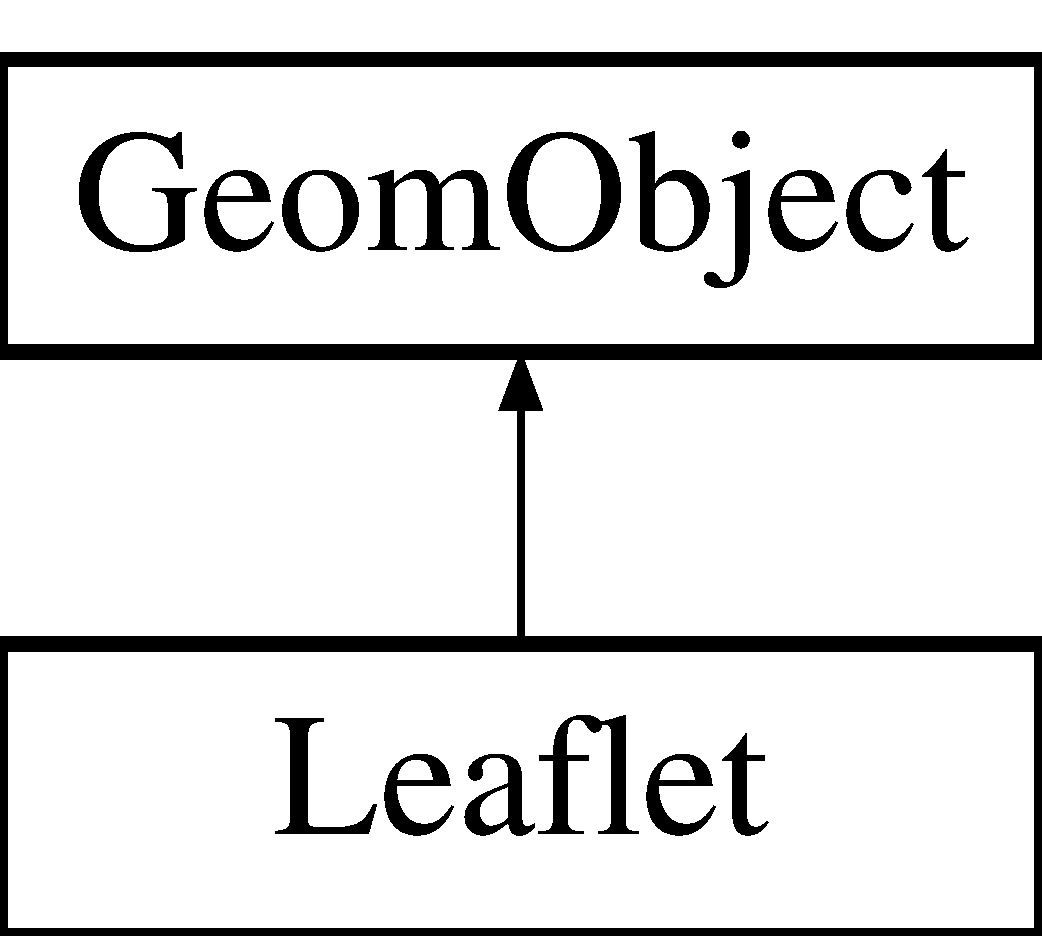
\includegraphics[height=2.000000cm]{classLeaflet}
\end{center}
\end{figure}
\subsection*{Public Member Functions}
\begin{DoxyCompactItemize}
\item 
\hyperlink{classLeaflet_acb53ccf4578a9981216cf0afd4b38453}{Leaflet} (const double \&\hyperlink{classLeaflet_a7a28827b7081107ac9e33087598ca868}{length}, const double \&\hyperlink{classLeaflet_a48e4d16790ffd9de527093eac8ff566c}{d\+\_\+x}, const double \&\hyperlink{classLeaflet_a8ff8044a3da540c7c9d7a89790b6ee58}{d\+\_\+y}, const double \&\hyperlink{classLeaflet_af4a819a3ba64960f4b796dc5a0d3eb5b}{x\+\_\+0}, const double \&period, Time $\ast$time\+\_\+pt)
\begin{DoxyCompactList}\small\item\em Constructor\+: Pass length (in Lagrangian coordinates), the amplitude of the horizontal and vertical deflection of the tip, the x-\/coordinate of the origin and the period of the oscillation. Passes the number of Lagrangian and Eulerian coordinates to the constructor of the Geom\+Object base class. \end{DoxyCompactList}\item 
virtual \hyperlink{classLeaflet_a0bbfaeec2534389b203fd2a2316db859}{$\sim$\+Leaflet} ()
\begin{DoxyCompactList}\small\item\em Destructor -- emtpy. \end{DoxyCompactList}\item 
void \hyperlink{classLeaflet_a5b78c2735652b6a5c08c6aa9d38b6232}{position} (const unsigned \&t, const Vector$<$ double $>$ \&xi, Vector$<$ double $>$ \&r) const
\begin{DoxyCompactList}\small\item\em Position vector, r, to the point identified by its 1D Lagrangian coordinate, xi (passed as a 1D Vector) at discrete time level t (t=0\+: present; t$>$0\+: previous). \end{DoxyCompactList}\item 
void \hyperlink{classLeaflet_a01daf4944eaaf7e9697eac53d78965f5}{position} (const Vector$<$ double $>$ \&xi, Vector$<$ double $>$ \&r) const
\begin{DoxyCompactList}\small\item\em Steady version\+: Get current shape. \end{DoxyCompactList}\item 
unsigned \hyperlink{classLeaflet_a91f2460718ec5a4ef32e302b8b14cdca}{ngeom\+\_\+data} () const
\begin{DoxyCompactList}\small\item\em Number of geometric Data in Geom\+Object\+: None. \end{DoxyCompactList}\item 
double \hyperlink{classLeaflet_a7a28827b7081107ac9e33087598ca868}{length} ()
\begin{DoxyCompactList}\small\item\em Length of the leaflet. \end{DoxyCompactList}\item 
double \& \hyperlink{classLeaflet_a48e4d16790ffd9de527093eac8ff566c}{d\+\_\+x} ()
\begin{DoxyCompactList}\small\item\em Amplitude of horizontal tip displacement. \end{DoxyCompactList}\item 
double \hyperlink{classLeaflet_a8ff8044a3da540c7c9d7a89790b6ee58}{d\+\_\+y} ()
\begin{DoxyCompactList}\small\item\em Amplitude of vertical tip displacement. \end{DoxyCompactList}\item 
double \hyperlink{classLeaflet_af4a819a3ba64960f4b796dc5a0d3eb5b}{x\+\_\+0} ()
\begin{DoxyCompactList}\small\item\em x-\/coordinate of leaflet origin \end{DoxyCompactList}\end{DoxyCompactItemize}
\subsection*{Private Attributes}
\begin{DoxyCompactItemize}
\item 
double \hyperlink{classLeaflet_a64c27b796ceece358d09d137f15bbf20}{Length}
\begin{DoxyCompactList}\small\item\em Length in terms of Lagrangian coordinates. \end{DoxyCompactList}\item 
double \hyperlink{classLeaflet_a473b6f4ef98bfba9e2c6974027ba4f4b}{D\+\_\+x}
\begin{DoxyCompactList}\small\item\em Horizontal displacement of tip. \end{DoxyCompactList}\item 
double \hyperlink{classLeaflet_af9c75c7aeecae4b14f7ba0fb245eb8ee}{D\+\_\+y}
\begin{DoxyCompactList}\small\item\em Vertical displacement of tip. \end{DoxyCompactList}\item 
double \hyperlink{classLeaflet_a29a25366a0cf97ad0dd36172fdfa3d0c}{X\+\_\+0}
\begin{DoxyCompactList}\small\item\em Origin. \end{DoxyCompactList}\item 
double \hyperlink{classLeaflet_a0d78b5fb3ec71009d4a9bcc79f8a85a9}{T}
\begin{DoxyCompactList}\small\item\em Period of the oscillations. \end{DoxyCompactList}\item 
Time $\ast$ \hyperlink{classLeaflet_ac10f13ad45456dc714ab57042861de53}{Time\+\_\+pt}
\begin{DoxyCompactList}\small\item\em Pointer to the global time object. \end{DoxyCompactList}\end{DoxyCompactItemize}


\subsection{Detailed Description}
Geom\+Object representing a vertical leaflet that performs bending and stretching oscillations. 

Definition at line 47 of file channel\+\_\+with\+\_\+leaflet.\+cc.



\subsection{Constructor \& Destructor Documentation}
\mbox{\Hypertarget{classLeaflet_acb53ccf4578a9981216cf0afd4b38453}\label{classLeaflet_acb53ccf4578a9981216cf0afd4b38453}} 
\index{Leaflet@{Leaflet}!Leaflet@{Leaflet}}
\index{Leaflet@{Leaflet}!Leaflet@{Leaflet}}
\subsubsection{\texorpdfstring{Leaflet()}{Leaflet()}}
{\footnotesize\ttfamily Leaflet\+::\+Leaflet (\begin{DoxyParamCaption}\item[{const double \&}]{length,  }\item[{const double \&}]{d\+\_\+x,  }\item[{const double \&}]{d\+\_\+y,  }\item[{const double \&}]{x\+\_\+0,  }\item[{const double \&}]{period,  }\item[{Time $\ast$}]{time\+\_\+pt }\end{DoxyParamCaption})\hspace{0.3cm}{\ttfamily [inline]}}



Constructor\+: Pass length (in Lagrangian coordinates), the amplitude of the horizontal and vertical deflection of the tip, the x-\/coordinate of the origin and the period of the oscillation. Passes the number of Lagrangian and Eulerian coordinates to the constructor of the Geom\+Object base class. 



Definition at line 57 of file channel\+\_\+with\+\_\+leaflet.\+cc.

\mbox{\Hypertarget{classLeaflet_a0bbfaeec2534389b203fd2a2316db859}\label{classLeaflet_a0bbfaeec2534389b203fd2a2316db859}} 
\index{Leaflet@{Leaflet}!````~Leaflet@{$\sim$\+Leaflet}}
\index{````~Leaflet@{$\sim$\+Leaflet}!Leaflet@{Leaflet}}
\subsubsection{\texorpdfstring{$\sim$\+Leaflet()}{~Leaflet()}}
{\footnotesize\ttfamily virtual Leaflet\+::$\sim$\+Leaflet (\begin{DoxyParamCaption}{ }\end{DoxyParamCaption})\hspace{0.3cm}{\ttfamily [inline]}, {\ttfamily [virtual]}}



Destructor -- emtpy. 



Definition at line 64 of file channel\+\_\+with\+\_\+leaflet.\+cc.



\subsection{Member Function Documentation}
\mbox{\Hypertarget{classLeaflet_a48e4d16790ffd9de527093eac8ff566c}\label{classLeaflet_a48e4d16790ffd9de527093eac8ff566c}} 
\index{Leaflet@{Leaflet}!d\+\_\+x@{d\+\_\+x}}
\index{d\+\_\+x@{d\+\_\+x}!Leaflet@{Leaflet}}
\subsubsection{\texorpdfstring{d\+\_\+x()}{d\_x()}}
{\footnotesize\ttfamily double\& Leaflet\+::d\+\_\+x (\begin{DoxyParamCaption}{ }\end{DoxyParamCaption})\hspace{0.3cm}{\ttfamily [inline]}}



Amplitude of horizontal tip displacement. 



Definition at line 92 of file channel\+\_\+with\+\_\+leaflet.\+cc.

\mbox{\Hypertarget{classLeaflet_a8ff8044a3da540c7c9d7a89790b6ee58}\label{classLeaflet_a8ff8044a3da540c7c9d7a89790b6ee58}} 
\index{Leaflet@{Leaflet}!d\+\_\+y@{d\+\_\+y}}
\index{d\+\_\+y@{d\+\_\+y}!Leaflet@{Leaflet}}
\subsubsection{\texorpdfstring{d\+\_\+y()}{d\_y()}}
{\footnotesize\ttfamily double Leaflet\+::d\+\_\+y (\begin{DoxyParamCaption}{ }\end{DoxyParamCaption})\hspace{0.3cm}{\ttfamily [inline]}}



Amplitude of vertical tip displacement. 



Definition at line 95 of file channel\+\_\+with\+\_\+leaflet.\+cc.

\mbox{\Hypertarget{classLeaflet_a7a28827b7081107ac9e33087598ca868}\label{classLeaflet_a7a28827b7081107ac9e33087598ca868}} 
\index{Leaflet@{Leaflet}!length@{length}}
\index{length@{length}!Leaflet@{Leaflet}}
\subsubsection{\texorpdfstring{length()}{length()}}
{\footnotesize\ttfamily double Leaflet\+::length (\begin{DoxyParamCaption}{ }\end{DoxyParamCaption})\hspace{0.3cm}{\ttfamily [inline]}}



Length of the leaflet. 



Definition at line 89 of file channel\+\_\+with\+\_\+leaflet.\+cc.

\mbox{\Hypertarget{classLeaflet_a91f2460718ec5a4ef32e302b8b14cdca}\label{classLeaflet_a91f2460718ec5a4ef32e302b8b14cdca}} 
\index{Leaflet@{Leaflet}!ngeom\+\_\+data@{ngeom\+\_\+data}}
\index{ngeom\+\_\+data@{ngeom\+\_\+data}!Leaflet@{Leaflet}}
\subsubsection{\texorpdfstring{ngeom\+\_\+data()}{ngeom\_data()}}
{\footnotesize\ttfamily unsigned Leaflet\+::ngeom\+\_\+data (\begin{DoxyParamCaption}{ }\end{DoxyParamCaption}) const\hspace{0.3cm}{\ttfamily [inline]}}



Number of geometric Data in Geom\+Object\+: None. 



Definition at line 86 of file channel\+\_\+with\+\_\+leaflet.\+cc.

\mbox{\Hypertarget{classLeaflet_a5b78c2735652b6a5c08c6aa9d38b6232}\label{classLeaflet_a5b78c2735652b6a5c08c6aa9d38b6232}} 
\index{Leaflet@{Leaflet}!position@{position}}
\index{position@{position}!Leaflet@{Leaflet}}
\subsubsection{\texorpdfstring{position()}{position()}\hspace{0.1cm}{\footnotesize\ttfamily [1/2]}}
{\footnotesize\ttfamily void Leaflet\+::position (\begin{DoxyParamCaption}\item[{const unsigned \&}]{t,  }\item[{const Vector$<$ double $>$ \&}]{xi,  }\item[{Vector$<$ double $>$ \&}]{r }\end{DoxyParamCaption}) const\hspace{0.3cm}{\ttfamily [inline]}}



Position vector, r, to the point identified by its 1D Lagrangian coordinate, xi (passed as a 1D Vector) at discrete time level t (t=0\+: present; t$>$0\+: previous). 



Definition at line 69 of file channel\+\_\+with\+\_\+leaflet.\+cc.

\mbox{\Hypertarget{classLeaflet_a01daf4944eaaf7e9697eac53d78965f5}\label{classLeaflet_a01daf4944eaaf7e9697eac53d78965f5}} 
\index{Leaflet@{Leaflet}!position@{position}}
\index{position@{position}!Leaflet@{Leaflet}}
\subsubsection{\texorpdfstring{position()}{position()}\hspace{0.1cm}{\footnotesize\ttfamily [2/2]}}
{\footnotesize\ttfamily void Leaflet\+::position (\begin{DoxyParamCaption}\item[{const Vector$<$ double $>$ \&}]{xi,  }\item[{Vector$<$ double $>$ \&}]{r }\end{DoxyParamCaption}) const\hspace{0.3cm}{\ttfamily [inline]}}



Steady version\+: Get current shape. 



Definition at line 80 of file channel\+\_\+with\+\_\+leaflet.\+cc.

\mbox{\Hypertarget{classLeaflet_af4a819a3ba64960f4b796dc5a0d3eb5b}\label{classLeaflet_af4a819a3ba64960f4b796dc5a0d3eb5b}} 
\index{Leaflet@{Leaflet}!x\+\_\+0@{x\+\_\+0}}
\index{x\+\_\+0@{x\+\_\+0}!Leaflet@{Leaflet}}
\subsubsection{\texorpdfstring{x\+\_\+0()}{x\_0()}}
{\footnotesize\ttfamily double Leaflet\+::x\+\_\+0 (\begin{DoxyParamCaption}{ }\end{DoxyParamCaption})\hspace{0.3cm}{\ttfamily [inline]}}



x-\/coordinate of leaflet origin 



Definition at line 98 of file channel\+\_\+with\+\_\+leaflet.\+cc.



\subsection{Member Data Documentation}
\mbox{\Hypertarget{classLeaflet_a473b6f4ef98bfba9e2c6974027ba4f4b}\label{classLeaflet_a473b6f4ef98bfba9e2c6974027ba4f4b}} 
\index{Leaflet@{Leaflet}!D\+\_\+x@{D\+\_\+x}}
\index{D\+\_\+x@{D\+\_\+x}!Leaflet@{Leaflet}}
\subsubsection{\texorpdfstring{D\+\_\+x}{D\_x}}
{\footnotesize\ttfamily double Leaflet\+::\+D\+\_\+x\hspace{0.3cm}{\ttfamily [private]}}



Horizontal displacement of tip. 



Definition at line 106 of file channel\+\_\+with\+\_\+leaflet.\+cc.

\mbox{\Hypertarget{classLeaflet_af9c75c7aeecae4b14f7ba0fb245eb8ee}\label{classLeaflet_af9c75c7aeecae4b14f7ba0fb245eb8ee}} 
\index{Leaflet@{Leaflet}!D\+\_\+y@{D\+\_\+y}}
\index{D\+\_\+y@{D\+\_\+y}!Leaflet@{Leaflet}}
\subsubsection{\texorpdfstring{D\+\_\+y}{D\_y}}
{\footnotesize\ttfamily double Leaflet\+::\+D\+\_\+y\hspace{0.3cm}{\ttfamily [private]}}



Vertical displacement of tip. 



Definition at line 109 of file channel\+\_\+with\+\_\+leaflet.\+cc.

\mbox{\Hypertarget{classLeaflet_a64c27b796ceece358d09d137f15bbf20}\label{classLeaflet_a64c27b796ceece358d09d137f15bbf20}} 
\index{Leaflet@{Leaflet}!Length@{Length}}
\index{Length@{Length}!Leaflet@{Leaflet}}
\subsubsection{\texorpdfstring{Length}{Length}}
{\footnotesize\ttfamily double Leaflet\+::\+Length\hspace{0.3cm}{\ttfamily [private]}}



Length in terms of Lagrangian coordinates. 



Definition at line 103 of file channel\+\_\+with\+\_\+leaflet.\+cc.

\mbox{\Hypertarget{classLeaflet_a0d78b5fb3ec71009d4a9bcc79f8a85a9}\label{classLeaflet_a0d78b5fb3ec71009d4a9bcc79f8a85a9}} 
\index{Leaflet@{Leaflet}!T@{T}}
\index{T@{T}!Leaflet@{Leaflet}}
\subsubsection{\texorpdfstring{T}{T}}
{\footnotesize\ttfamily double Leaflet\+::T\hspace{0.3cm}{\ttfamily [private]}}



Period of the oscillations. 



Definition at line 115 of file channel\+\_\+with\+\_\+leaflet.\+cc.

\mbox{\Hypertarget{classLeaflet_ac10f13ad45456dc714ab57042861de53}\label{classLeaflet_ac10f13ad45456dc714ab57042861de53}} 
\index{Leaflet@{Leaflet}!Time\+\_\+pt@{Time\+\_\+pt}}
\index{Time\+\_\+pt@{Time\+\_\+pt}!Leaflet@{Leaflet}}
\subsubsection{\texorpdfstring{Time\+\_\+pt}{Time\_pt}}
{\footnotesize\ttfamily Time$\ast$ Leaflet\+::\+Time\+\_\+pt\hspace{0.3cm}{\ttfamily [private]}}



Pointer to the global time object. 



Definition at line 118 of file channel\+\_\+with\+\_\+leaflet.\+cc.

\mbox{\Hypertarget{classLeaflet_a29a25366a0cf97ad0dd36172fdfa3d0c}\label{classLeaflet_a29a25366a0cf97ad0dd36172fdfa3d0c}} 
\index{Leaflet@{Leaflet}!X\+\_\+0@{X\+\_\+0}}
\index{X\+\_\+0@{X\+\_\+0}!Leaflet@{Leaflet}}
\subsubsection{\texorpdfstring{X\+\_\+0}{X\_0}}
{\footnotesize\ttfamily double Leaflet\+::\+X\+\_\+0\hspace{0.3cm}{\ttfamily [private]}}



Origin. 



Definition at line 112 of file channel\+\_\+with\+\_\+leaflet.\+cc.



The documentation for this class was generated from the following file\+:\begin{DoxyCompactItemize}
\item 
\hyperlink{channel__with__leaflet_8cc}{channel\+\_\+with\+\_\+leaflet.\+cc}\end{DoxyCompactItemize}

\chapter{File Documentation}
\hypertarget{channel__with__leaflet_8cc}{}\section{channel\+\_\+with\+\_\+leaflet.\+cc File Reference}
\label{channel__with__leaflet_8cc}\index{channel\+\_\+with\+\_\+leaflet.\+cc@{channel\+\_\+with\+\_\+leaflet.\+cc}}
\subsection*{Classes}
\begin{DoxyCompactItemize}
\item 
class \hyperlink{classLeaflet}{Leaflet}
\item 
class \hyperlink{classChannelWithLeafletProblem}{Channel\+With\+Leaflet\+Problem$<$ E\+L\+E\+M\+E\+N\+T $>$}
\begin{DoxyCompactList}\small\item\em Problem class. \end{DoxyCompactList}\end{DoxyCompactItemize}
\subsection*{Namespaces}
\begin{DoxyCompactItemize}
\item 
 \hyperlink{namespaceGlobal__Physical__Variables}{Global\+\_\+\+Physical\+\_\+\+Variables}
\begin{DoxyCompactList}\small\item\em Global parameters. \end{DoxyCompactList}\end{DoxyCompactItemize}
\subsection*{Functions}
\begin{DoxyCompactItemize}
\item 
int \hyperlink{channel__with__leaflet_8cc_a0ddf1224851353fc92bfbff6f499fa97}{main} (int argc, char $\ast$argv\mbox{[}$\,$\mbox{]})
\end{DoxyCompactItemize}
\subsection*{Variables}
\begin{DoxyCompactItemize}
\item 
double \hyperlink{namespaceGlobal__Physical__Variables_ab814e627d2eb5bc50318879d19ab16b9}{Global\+\_\+\+Physical\+\_\+\+Variables\+::\+Re} =20.\+0
\begin{DoxyCompactList}\small\item\em Reynolds number. \end{DoxyCompactList}\end{DoxyCompactItemize}


\subsection{Function Documentation}
\mbox{\Hypertarget{channel__with__leaflet_8cc_a0ddf1224851353fc92bfbff6f499fa97}\label{channel__with__leaflet_8cc_a0ddf1224851353fc92bfbff6f499fa97}} 
\index{channel\+\_\+with\+\_\+leaflet.\+cc@{channel\+\_\+with\+\_\+leaflet.\+cc}!main@{main}}
\index{main@{main}!channel\+\_\+with\+\_\+leaflet.\+cc@{channel\+\_\+with\+\_\+leaflet.\+cc}}
\subsubsection{\texorpdfstring{main()}{main()}}
{\footnotesize\ttfamily int main (\begin{DoxyParamCaption}\item[{int}]{argc,  }\item[{char $\ast$}]{argv\mbox{[}$\,$\mbox{]} }\end{DoxyParamCaption})}

Driver code -- pass a command line argument if you want to run the code in validation mode where it only performs a few steps Initialise timestep

Set max. number of adaptations (reduced for validation)

Output steady solution

Reduce the max number of adaptations for time-\/dependent simulation 

Definition at line 390 of file channel\+\_\+with\+\_\+leaflet.\+cc.



References Channel\+With\+Leaflet\+Problem$<$ E\+L\+E\+M\+E\+N\+T $>$\+::doc\+\_\+solution().


\hypertarget{channel__with__leaflet_8txt__doxygenified_8h}{}\section{channel\+\_\+with\+\_\+leaflet.\+txt\+\_\+doxygenified.\+h File Reference}
\label{channel__with__leaflet_8txt__doxygenified_8h}\index{channel\+\_\+with\+\_\+leaflet.\+txt\+\_\+doxygenified.\+h@{channel\+\_\+with\+\_\+leaflet.\+txt\+\_\+doxygenified.\+h}}

%--- End generated contents ---

% Index
\backmatter
\newpage
\phantomsection
\clearemptydoublepage
\addcontentsline{toc}{chapter}{Index}
\printindex

\end{document}
